\section{物体的热膨胀}\label{sec:2-1}

\begin{wrapfigure}[10]{r}{6cm}
    \centering
    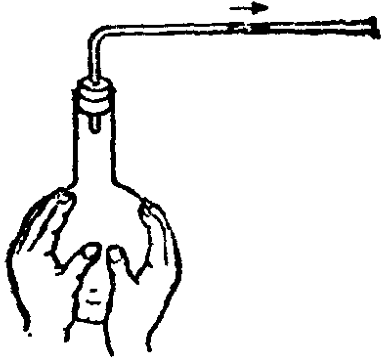
\includegraphics[width=5cm]{../pic/czwl2-ch2-1}
    \caption{气体的热膨胀}\label{fig:2-1}
\end{wrapfigure}

\xiaobiaoti{气体的热膨胀}
把一根弯成直角的玻璃管穿过软木塞插进烧瓶里,
在水平部分的玻璃管里预先装有一段带色的小水柱(图 \ref{fig:2-1})。
被小水柱密封在烧瓶里的空气就是我们要研究的气体。
空气体积的变化,可以从小水柱在玻璃管里的移动看出来。

用手握着烧瓶,使烧瓶里的空气变热,温度升高,就会看到玻璃管里的小水柱向右移动。
这表明空气在温度升高的时候膨胀,体积增大。
手离开后,烧瓶里的空气温度降低,这时小水柱向左移动。
这表明空气在温度降低的时候收缩,体积减小。

在上面的实验里,如果烧瓶里装的不是空气,而是别的任何一种气体,结果也是一样。
因此得到下面的结论:

\CJKunderwave{气体在温度升高的时候膨胀,在温度降低的时候收缩}。


\begin{figure}[htbp]
    \centering
    \begin{minipage}{6cm}
    \centering
    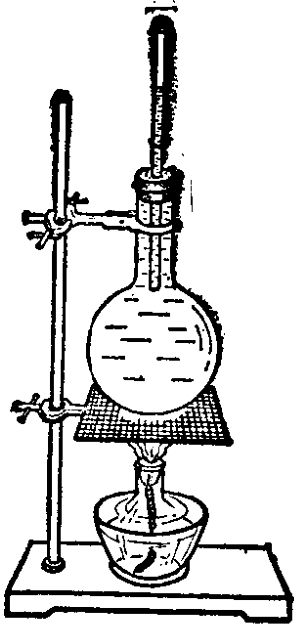
\includegraphics[width=4cm]{../pic/czwl2-ch2-2}
    \caption{液体的热膨胀}\label{fig:2-2}
    \end{minipage}
    \qquad
    \begin{minipage}{8cm}
    \centering
    \vspace{5.5cm}
    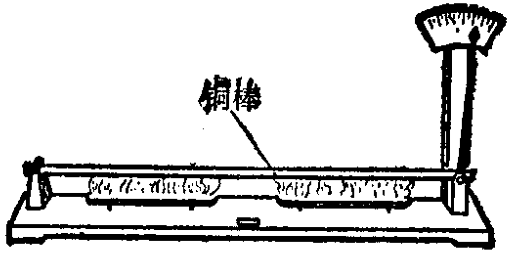
\includegraphics[width=6cm]{../pic/czwl2-ch2-3}
    \caption{固体的热膨胀}\label{fig:2-3}
    \end{minipage}
\end{figure}

\xiaobiaoti{液体的热膨胀}
液体在温度改变的时候,体积也要发生变化。

在烧瓶里装满水或者别的液体,用插有玻璃管的软木塞把瓶口塞紧,液面就升到玻璃管里。
在玻璃管上套上橡皮环,标出这时液面的位置。
对烧瓶加热,使瓶里液体的温度升高,就会看到玻璃管里的液面上升(图 \ref{fig:2-2})。
停止加热,瓶里的液体温度降低,液面又下降。

可见,\CJKunderwave{液体在温度升高的时候膨胀,在温度降低的时候收缩}。

\xiaobiaoti{固体的热膨胀}
如图 \ref{fig:2-3} 所示,铜棒的左端固定,右端放在转轴上,转轴上装着指针。
给铜棒加热,它的温度升高,可以看到指针向右偏,这表明铜棒膨胀了。
停止加热,并在铜棒上盖上浸过冷水的毛巾,使它的温度降低,指针向左偏,这表明铜棒收缩了。
换用其他材料的棒来做这个实验,可以看到同样的现象。

可见,\CJKunderwave{固体在温度升高的时候膨胀,在温度降低的时候收缩}。


在上述实验里,要看出热膨胀现象,
对于气体只要用手加热,气体的温度变化不大;
对于液体要用酒精灯烧,液体的温度变化较大;
对于固体不但要烧,而且要利用指针的偏转把膨胀放大。
这说明气体的热膨胀最显著,液体的热膨胀不如气体显著,固体的热膨胀最不显著。


对于气体、液体和固体的热膨胀,我们得出下面的结论:

\textbf{一般物体都是在温度升高的时候膨胀,在温度降低的时候收缩。
在相同的条件下,固体膨胀得最小,液体膨胀得较大,气体膨胀得最大}。

